\documentclass[11pt,a4paper,openany]{book}
\usepackage[margin=24mm]{geometry}
\usepackage{fontspec}
\IfFontExistsTF{Noto Serif}{\setmainfont{Noto Serif}}{\setmainfont{DejaVu Serif}}
\usepackage{amsmath,amssymb}
\usepackage{tikz}
\usepackage{enumitem}
\usepackage{microtype}
\usepackage[hidelinks]{hyperref}
\setlength{\parindent}{0pt}
\setlength{\parskip}{5pt}
\setlist[enumerate]{leftmargin=*,itemsep=9pt}

\renewcommand{\contentsname}{Contents}
\begin{document}
\title{V-TALENT 2045\\ PHY202-A --- Newtonian dynamics, friction and constraints\\\large Level 2 · Advanced mechanics · Grades 10–12}
\author{Dr. Dang Minh Tuan -- TS. Đặng Minh Tuấn}
\date{2026 · v1.0}
\maketitle
\tableofcontents
\chapter*{Learning objectives}\addcontentsline{toc}{chapter}{Learning objectives}
Derive equations from free-body diagrams; determine static-friction regimes, solve constrained dynamics, derive rolling conditions and test limiting cases. Prepare for multi-regime VPhO/TST problems.

First subject booklet, draft 1.0. Original problems; external archive references are for further study, not reproduced. Independently review before formal assessment.
\chapter{Newton's laws and piecewise friction}
\section{Theory and derivations}
Choose a system, inertial frame and coordinate axes. Newton's second law $\sum\vec F_{\rm ext}=d\vec p/dt$ reduces to $m\vec a$ for a constant-mass particle. Internal forces cancel in the equation for total momentum, but may determine relative motion and internal energy. For a non-inertial translating frame with acceleration $\vec A$, introduce the inertial force $-m\vec A$; do not mix accelerations from different frames in the same equation. A force diagram represents forces acting on one chosen body, not all interaction partners.

Coulomb friction is a model: $|f_s|\le\mu_s N$ while the surfaces stick, and $|f_k|=\mu_k N$ during sliding, opposite relative slip. Static friction is a constraint reaction, not automatically $\mu_sN$. Determine $N$ from the perpendicular dynamics; it need not equal $mg$. Assume sticking, solve for the required friction, and compare its magnitude with $\mu_sN$. If infeasible, determine the slip direction and solve again using kinetic friction. At $N=0$ the contact model must be reconsidered.

For two blocks $m$ above $M$ on a smooth floor, horizontal force $F$ on the lower block and no vertical acceleration, sticking gives $a=F/(M+m)$ and upper-block friction $f=ma$. Thus $F\le\mu_s(M+m)g$. Above that threshold (with forward slip of the lower block), the upper block has $a_m=\mu_k g$ and the lower block $a_M=(F-\mu_k mg)/M$. Check $a_M>a_m$ to confirm the assumed slip. This piecewise structure is typical of Olympiad questions.

If a force $F$ makes angle $\theta$ above horizontal on a block remaining in contact with a flat floor, $N=mg-F\sin\theta$. In forward sliding $a=[F(\cos\theta+\mu_k\sin\theta)-\mu_kmg]/m$. The formal optimum is $\tan\theta=\mu_k$ for $0\le\theta\le\pi/2$, but only when contact remains and the forward-sliding regime is valid. Thus optimization follows model selection, not the reverse.
\begin{center}
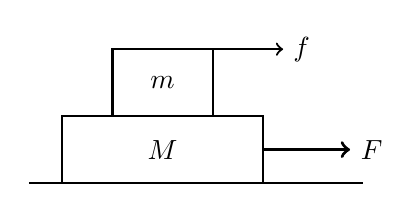
\begin{tikzpicture}[scale=.85]
\draw[thick] (-2,-1.8)--(3,-1.8);
\draw[thick] (-1.5,-1.8) rectangle (1.5,-.8);
\draw[thick] (-.75,-.8) rectangle (.75,.2);
\node at (0,-1.3) {$M$};\node at (0,-.3) {$m$};
\draw[->,very thick] (1.5,-1.3)--(2.8,-1.3) node[right] {$F$};
\draw[->,thick] (0,.2)--(1.8,.2) node[right] {$f$};
\end{tikzpicture}
\end{center}
\section{Worked example}
\subsection*{Worked example 1.1}
Two blocks: upper 2 kg, lower 3 kg, smooth floor. A horizontal force on the lower block is gradually increased. Use g=10 m/s\textsuperscript{2}, μs=0.4, μk=0.3. Find the threshold and both accelerations at 15 N and 30 N.

\textbf{Solution.} Sticking requires $f=2F/5\le0.4(2)(10)=8$ N, hence $F_c=20$ N. At 15 N, $a=15/5=3$ m/s\textsuperscript{2} and $f=6$ N, feasible. At 30 N the sticking demand is 12 N, impossible. Kinetic friction is 6 N, forward on the upper body: $a_m=6/2=3$ m/s\textsuperscript{2}. Backward on lower: $a_M=(30-6)/3=8$ m/s\textsuperscript{2}. Since $8>3$ the slip direction is consistent. Total momentum check: $2(3)+3(8)=30$ N.
\subsection*{Worked example 1.2}
A 4 kg block is already sliding on a horizontal surface. A 20 N force pulls at an angle θ above horizontal, μk=0.25, g=10. Determine the angle giving maximum forward acceleration, and verify contact.

\textbf{Solution.} For forward slip, $N=40-20\sin\theta>0$ for every allowed angle. The acceleration is $a=[20(\cos\theta+0.25\sin\theta)-10]/4$. Write $\cos\theta+0.25\sin\theta=\sqrt{1+0.25^2}\cos(\theta-\arctan0.25)$. Hence $\theta=\arctan0.25\approx14.04^\circ$ and $a_{\max}=[20\sqrt{1.0625}-10]/4\approx2.654$ m/s\textsuperscript{2}. At the optimum $N\approx35.15$ N. This applies while sliding forward.
\section{End-of-topic practice}
\begin{enumerate}
\item \textbf{PHY202-A-1.1}. Upper mass 1 kg, lower 4 kg; smooth floor, μs=0.5, μk=0.3, g=10. Force on lower block: 20 N, then 40 N. Determine each acceleration in the two cases.
\item \textbf{PHY202-A-1.2}. Repeat the two-block threshold derivation when horizontal force F is applied to the upper mass m instead. Lower mass M is on a smooth floor.
\item \textbf{PHY202-A-1.3}. A 5 kg crate on a 30\textdegree{} incline has μs=0.4 and μk=0.3. Starting from rest without an applied force, determine whether it slips and its acceleration if it does. g=10.
\item \textbf{PHY202-A-1.4}. A block is at rest on a horizontal accelerating truck bed. Derive the minimum μs required to prevent slip when truck acceleration is A. Explain from both frames.
\end{enumerate}
\chapter{Constraints, pulleys and rolling}
\section{Theory and derivations}
For a taut inextensible string, write a geometric length equation before using Newton's laws. For a fixed pulley with two vertical ends $y_1+y_2=L$ (both downward positive), differentiating twice gives $a_1+a_2=0$. A massless string over an ideal massless frictionless pulley has equal tension; a massive pulley requires distinct tensions to generate torque. The no-slip string constraint is $a=R\alpha$. These relations are independent of Newton's laws and close the system of equations.

For an Atwood machine with $m_2>m_1$, pulley moment of inertia $I$, radius $R$, negligible axle friction, write $m_2g-T_2=m_2a$, $T_1-m_1g=m_1a$, $(T_2-T_1)R=I a/R$. Adding yields $a=(m_2-m_1)g/(m_1+m_2+I/R^2)$. The ratio $I/R^2$ has mass units and contributes rotational inertia, not weight. As $I\to0$, recover the ideal pulley; as $I$ grows, $a$ decreases.

A rigid axisymmetric body of mass $m$ and $I=\kappa mR^2$ rolls from rest down an incline $\theta$. With downslope translation and rolling angular acceleration positive, $mg\sin\theta-f=ma$ and $fR=I a/R$ yield $a=g\sin\theta/(1+\kappa)$, $f=\kappa mg\sin\theta/(1+\kappa)$ uphill. Required $\mu_s\ge\kappa\tan\theta/(1+\kappa)$. For pure rolling on a fixed rigid surface, the contact point is instantaneously at rest, so static friction does no work in the ground frame. The energy equation $mgh=(mv^2+I\omega^2)/2$ gives $v=\sqrt{2gh/(1+\kappa)}$. Energy alone cannot verify sufficient static friction.

\section{Worked example}
\subsection*{Worked example 2.1}
An Atwood machine has masses 2 and 5 kg and a uniform disk pulley of mass 4 kg. With g=10, find acceleration and the two tensions.

\textbf{Solution.} For a disk $I/R^2=M_p/2=2$ kg. The effective inertia is $2+5+2=9$ kg, driving force 30 N. Thus $a=10/3$ m/s\textsuperscript{2}. $T_1=2(10+10/3)=80/3$ N, $T_2=5(10-10/3)=100/3$ N. The difference $20/3$ N equals $(I/R^2)a=2(10/3)$, as required.
\subsection*{Worked example 2.2}
A uniform solid cylinder rolls from rest down a 30\textdegree{} incline of vertical height 1.2 m. Let g=10. Find a, v at the bottom and minimum μs.

\textbf{Solution.} $\kappa=1/2$ gives $a=5/1.5=10/3$ m/s\textsuperscript{2}. The path length is $1.2/\sin30^\circ=2.4$ m. Using $v^2=2as=16$, $v=4$ m/s. Energy confirms $2gh/(1+\kappa)=16$. Required $\mu_s=(1/3)\tan30^\circ=1/(3\sqrt3)\approx0.192$. Below this value the rolling-only model is invalid.
\section{Experimental investigation}
Use two cylinders of comparable radius but different mass distributions and a low ramp. Film each from rest; measure distance versus time, fit s against t\textsuperscript{2}, compare slope with g sinθ/[2(1+κ)]. Mark the rim and check v≈Rω from video; if slipping, do not interpret data as pure rolling. Report angle uncertainty, rolling resistance, timing and repeatability.
\section{End-of-topic practice}
\begin{enumerate}
\item \textbf{PHY202-A-2.1}. Atwood masses 3 kg and 7 kg, disk pulley mass 2 kg. Find a and tensions with g=10.
\item \textbf{PHY202-A-2.2}. A hoop and a solid sphere, same mass and radius, start from rest and roll without slipping down the same incline. Derive their acceleration ratio and their bottom-speed ratio.
\item \textbf{PHY202-A-2.3}. A solid cylinder is released on an incline with tan θ=0.6, μs=0.15 and μk=0.10. Decide whether pure rolling is possible. If not, find initial translational and angular accelerations in terms of g and R.
\item \textbf{PHY202-A-2.4}. A light movable pulley supports a 6 kg load by two vertical rope segments. The free end is pulled down 0.8 m at constant speed by an ideal arrangement. Find load displacement, tension and input work; g=10.
\end{enumerate}
\chapter*{Further study and sources}\addcontentsline{toc}{chapter}{Further study and sources}
VPhO 2001 group 1 item 1.1 (printed p. 5); VPhO 2003 group 5 item 5.1 (pp. 14–15); VPhO 2008 group 14 item 14.1 (p. 36); VN TST 2003 group 21 item 21.1 (pp. 56–58). These locators refer to the supplied collection, not original exercises in this booklet.

\url{https://diavn.github.io/truongchuyen/physics-vpho.html}

\url{https://hyperphysics.gsu.edu/hbase/hph.html}

\url{https://openstax.org/subjects/science}
\appendix
\chapter{Full solutions to practice}
\section{Newton's laws and piecewise friction}
\begin{enumerate}
\item \textbf{PHY202-A-1.1}. Threshold $F_c=0.5(5)10=25$ N. At 20 N both accelerate at 4 m/s\textsuperscript{2}, requiring 4 N friction. At 40 N, $f_k=3$ N, $a_m=3$ m/s\textsuperscript{2} and $a_M=(40-3)/4=9.25$ m/s\textsuperscript{2}. The lower block moves ahead; total $1(3)+4(9.25)=40$ N.
\item \textbf{PHY202-A-1.2}. Sticking still gives $a=F/(M+m)$. Friction on the lower block must supply $Ma=MF/(M+m)$. Since $N=mg$, feasibility requires $MF/(M+m)\le\mu_smg$, i.e. $F_c=\mu_smg(M+m)/M$. Above threshold $a_M=\mu_kmg/M$ and $a_m=(F-\mu_kmg)/m$. The expression differs from force applied below because the driven partner differs.
\item \textbf{PHY202-A-1.3}. $N=mg\cos30^\circ=25\sqrt3$ N; downslope gravity $mg\sin30^\circ=25$ N. Maximum static friction $10\sqrt3\approx17.32$ N, insufficient. Kinetic friction $7.5\sqrt3$ N up the slope. Hence $a=(25-7.5\sqrt3)/5=5-1.5\sqrt3\approx2.40$ m/s\textsuperscript{2} down.
\item \textbf{PHY202-A-1.4}. Ground frame: required forward friction $f=mA$, $N=mg$, so $\mu_s\ge A/g$. Truck frame: the block is stationary, inertial force $-mA$ balances $f=mA$. Both frames give the same contact requirement. At equality slip is impending.
\end{enumerate}
\section{Constraints, pulleys and rolling}
\begin{enumerate}
\item \textbf{PHY202-A-2.1}. $I/R^2=1$ kg; $a=40/11$ m/s\textsuperscript{2}. $T_1=3(10+40/11)=450/11$ N and $T_2=7(10-40/11)=490/11$ N. Difference $40/11$ N supplies the pulley torque.
\item \textbf{PHY202-A-2.2}. $\kappa_h=1$, $\kappa_s=2/5$. Then $a_s/a_h=(1+1)/(1+2/5)=10/7$. At equal height drop, $v_s/v_h=\sqrt{10/7}$. Both results require enough static friction for each object.
\item \textbf{PHY202-A-2.3}. Pure rolling requires $\mu_s\ge\tan\theta/3=0.2$, so it fails. Gravity causes downslope contact slip, friction acts uphill. $\cos\theta=1/\sqrt{1.36}$ and $\sin\theta=0.6/\sqrt{1.36}$. Then $a=g(\sin\theta-0.1\cos\theta)=0.5g/\sqrt{1.36}$; $\alpha=fR/I=0.2g/(R\sqrt{1.36})$. Since $a-R\alpha=0.3g/\sqrt{1.36}>0$, the assumed slip is consistent.
\item \textbf{PHY202-A-2.4}. The rope length constraint is $2y+x=\text{constant}$ for downward load coordinate $y$ and free-end coordinate $x$. Thus $\Delta y=-0.4$ m: load rises 0.4 m. Constant speed gives $2T=mg=60$ N, so $T=30$ N. Input work $T(0.8)=24$ J, equal to $mgh=6(10)(0.4)=24$ J.
\end{enumerate}
\end{document}
